\documentclass[a4paper, 14pt]{extarticle}

\usepackage{../generalPreamble}
\usepackage{../reportFormat}


\begin{document}

\begin{titlepage}
    \centering
    {\bfseries
        \uppercase{
            Минобрнауки России \\
            Санкт-Петербургский государственный \\
            Электротехнический университет \\
            \enquote{ЛЭТИ} им. В.И.Ульянова (Ленина)\\
        }
        Кафедра ИБ

        \vspace{\fill}
        \uppercase{Лабораторная работа №4} \\
        по дисциплине \enquote{Криптография и защита информации} \\
        Тема: Изучение шифра DES
    }

    \vspace{\fill}
    \begin{tabularx}{0.8\textwidth}{l X c r}
        Студент гр. 6304 & & \underline{\hspace{3cm}} & Корытов П.В.\\
        Преподаватель & & \underline{\hspace{3cm}} & Племянников А.К.
    \end{tabularx}

    \vspace{1cm}
    Санкт-Петербург \\
    \the\year{}
\end{titlepage}

\newpage

\section*{Цель работы}
Цель работы: исследовать шифры Hill, ADFGVX, Playfair и получить практические навыки работы с ними, в том числе и в программном продукте CrypTool 1 и 2.

\section{Исследование преобразований DES}
\subsection{Описание}
DES (англ. Data Encryption Standart) --- стандарт шифрования данных --- блочный шифр с симетричными ключами. Разработан NIST (National Institute of Standarts and Technology).

\subsubsection{Сеть Фейстеля}
Шифр DES основан на сети Фейстеля (см. рисунок~\ref{img:1:1}). Принцип работы сети следующий:

\begin{figure}[h]
    \centering
    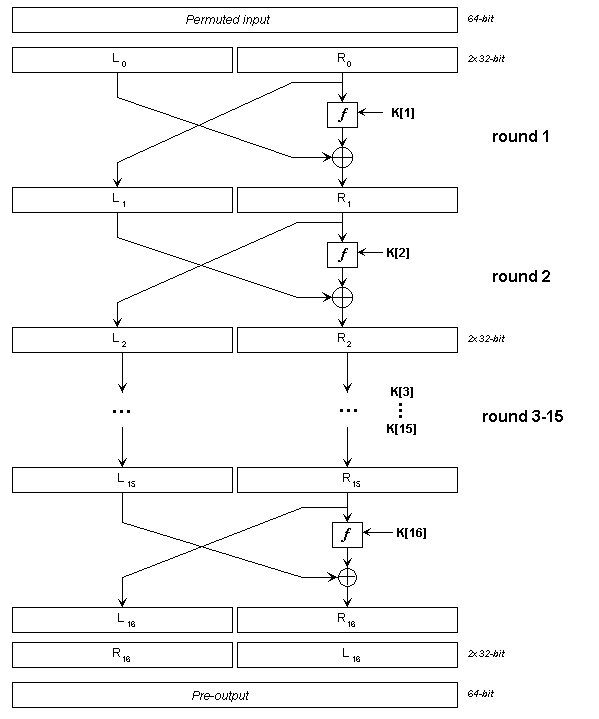
\includegraphics[width=0.6\textwidth]{./img/S001.jpg}
    \caption{Сеть Фейстеля}%
    \label{img:1:1}
\end{figure}

\begin{enumerate}
    \item Выбранный блок делится на два равных субблока $A_0$ и $B_0$
    \item $L_0$ преобразуется функцией шифра $f(A_0, K_0)$, после чего складывается по модулю 2 с $B_0$
    \item Результат сложения становится $B_1$, а $B_0$ становится $A_1$ для следующего раунда
    \item Операция повторяется $N-1$ раз. При переходе между раундами меняются раундовые ключи $K_0, K_1, \ldots $.\\
\end{enumerate}
Т.е.:
\[ A_i = B_{i-1}; \]
\[ B_i = A_{i-1} \oplus f(B_{i-1}), \] 
где $i$ --- номер текущего рауда, $K_i$ --- ключ раунда.

В шифре DES размер блока --- 64 бита, число раундов --- 16. Перед входом в сеть производится начальная перестановка.

\FloatBarrier{}

\subsubsection{Структура раудовой функции}
Структура функции представлена на рисунке~\ref{img:1:2}.
\begin{figure}[h]
    \centering
    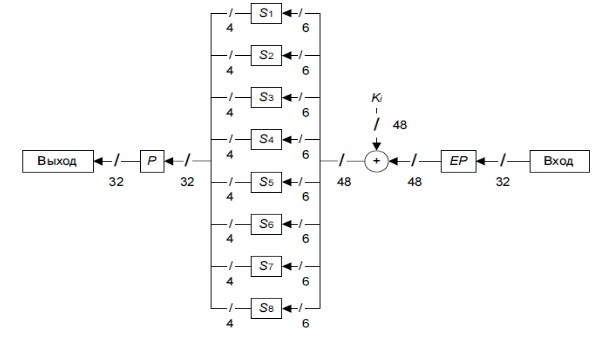
\includegraphics[width=0.9\textwidth]{./img/S002.jpg}
    \caption{Структура $f$}%
    \label{img:1:2}
\end{figure}

Этапы функции:
\begin{enumerate}
    \item Расширяющая перестановка, преобразует 32 бита в 48 бит (рисунок~\ref{img:1:3})
        \begin{figure}[h]
            \centering
            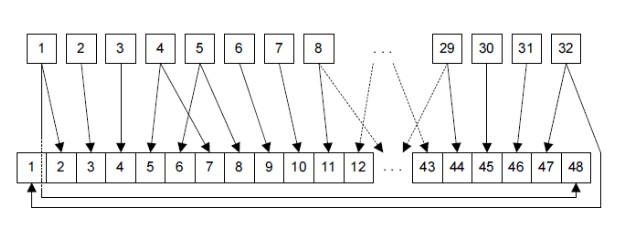
\includegraphics[width=0.9\textwidth]{./img/S003.jpg}
            \caption{Расширящая перестановка}%
            \label{img:1:3}
        \end{figure}
    \item Полученные 48 бит складываются с $K_i$ операцией xor
    \item Результат сложения разбивается на 8 блоков по 6 битов. Каждый блок обрабатывается соответствующей таблицей замен
    \item Над полученными 32 битами, после выполнения замен, выполняется перестановка ($P$)
\end{enumerate}

\subsubsection{Генерация раундовых ключей}
Генерация раундовых ключей представлена на рисунке~\ref{img:1:4}.
\begin{figure}[h]
    \centering
    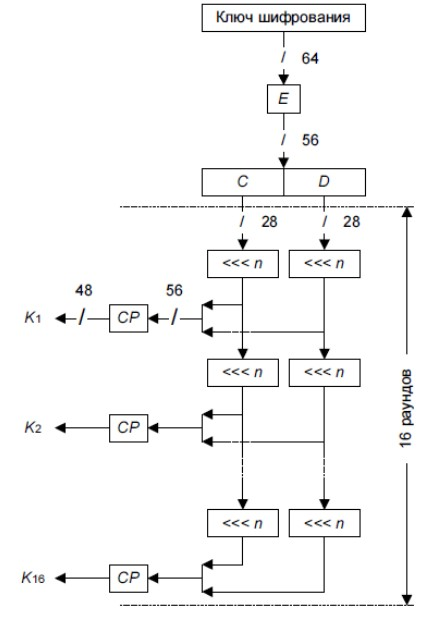
\includegraphics[width=0.7\textwidth]{./img/S004.jpg}
    \caption{Генерация раундовых ключей}%
    \label{img:1:4}
\end{figure}
Из 64-битного ключа используется только 56 бит --- каждый 8-й бит исключается. После выполняется перестановка ($E$).

После перестановки блок в 56 бит делится на два 28-битных блока ($C$, $D$). Затем выполняются 16 раудов преобразований:
\begin{enumerate}
    \item Текущие $C, D$ циклически сдвигаются влева на определенное количество бит
    \item $C, D$ объединяются в 56-битное значение, к которому применяется сжимающая перестановка $CP$. Получается 48-битный ключ.
\end{enumerate}


\FloatBarrier{}
\subsection{Формулировка задания}

\begin{itemize}
    \item Изучить преобразования шифра DES с помощью демонстрационного приложения из Cryptool 1.
        \begin{itemize}
            \item Indiv.Procedures-> Visualization…-> DES…
        \end{itemize}
    \item Выполнить вручную преобразования одного раунда и вычисление раундовых ключей при следующих исходных данных:
        \begin{itemize}
            \item Открытый текст (не более 64 бит) – фамилия\_имя (транслитерация латиницей)
            \item Ключ (56 бит) – номер зачетной книжки II инициал (всего 7 символов)
        \end{itemize}
    \item Выполнить вручную обратное преобразование зашифрованного сообщения
\end{itemize}

\subsection{Ход работы}
\lipsum[1] %TODO

\section{Исследование DES в режимах ECB и CBC}
\subsection{Описание}
Режим ECB (рис.~\ref{img:1:5}) шифра DES работает независимо с каждым 64-битным блоком шифруемых данных. Режим CBC (рис.~\ref{img:1:6}) перед запуском шифрования каждого очередного блока складывает его с предыдущим операцией xor

\begin{figure}[h]
    \centering
    \begin{subfigure}[b]{0.43\textwidth}
        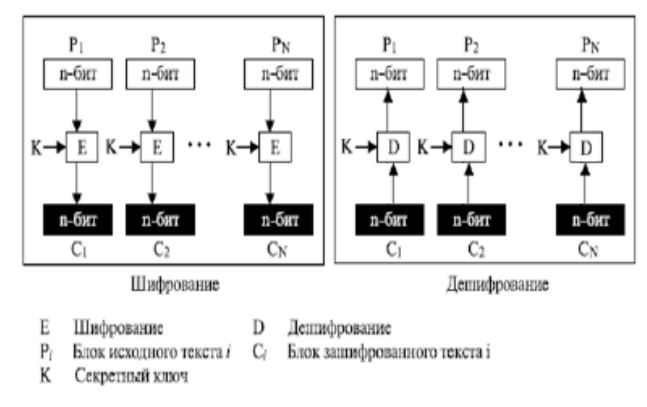
\includegraphics[width=\textwidth]{./img/S005.jpg}
        \caption{Режим ECB}%
        \label{img:1:5}
    \end{subfigure}%
    \hspace{2cm}
    \begin{subfigure}[b]{0.43\textwidth}
        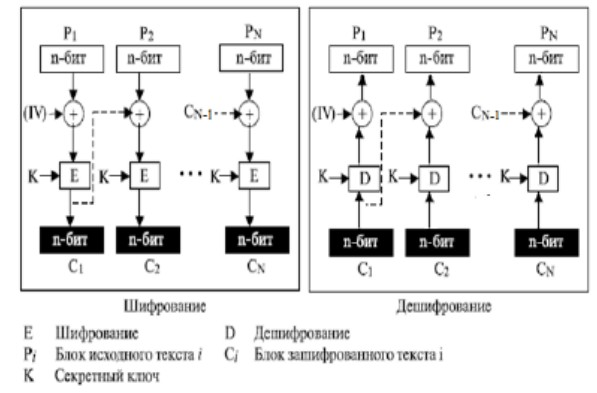
\includegraphics[width=\textwidth]{./img/S006.jpg}
        \caption{Режим CBC}%
        \label{img:1:6}
    \end{subfigure}
    \caption{Режимы DES}
\end{figure}


\subsection{Формулировка задания}
\begin{itemize}
    \item Создать картинку со своими ФИО (формат bmp).
    \item Зашифровать картинку шифром DES в режиме ECB.\@
    \item Зашифровать картинку шифром DES в режиме CBC c тем же ключом.
    \item Сохранить скриншоты картинок для отчета.
    \item Сжать исходную и 2 зашифрованных картинки средствами CrypTool. Зафиксировать размеры полученных файлов в таблице.
    \item Выбрать случайный текст на английском языке (не менее 1000 знаков) и зашифровать его DES в режиме ECB.\@
    \item Для одного и того же шифротекста оцените время проведения атаки «грубой силы» в случаях, когда известно n-4, n-6, n-8,.., 2 байт секретного ключа. Зафиксировать результаты измерений в таблице.
\end{itemize}

\section{Исследование 3-DES}
\subsection{Описание}
Шифр 3-DES состоит в трехкратном применении обычного шифра DES.\@ Существуют 4 основные версии этого шифра:
\begin{enumerate}
    \item \texttt{DES-EEE3} --- шифрование происходит 3 раза независимыми ключасми
    \item \texttt{DES-EDE3} --- операция шифровка-расшифровка-шифровка с тремя разными ключами
    \item \texttt{DES-EEE2} --- то же, что и \texttt{DES-EE3}, но на первом и последнем шаге одинаковый ключ
    \item \texttt{DES-EDE2} --- то же, что и \texttt{DES-EDE2}, но на первом и последнем шаге одинаковый ключ\\
\end{enumerate}
На текущий момент самыми популярными разновидностями шифра являются \texttt{DES-EDE3} и \texttt{DES-EDE2}.  

\subsection{Формулировка задания}
\begin{itemize}
    \item Выбрать случайный текст на английском языке (не менее 1000 знаков).
    \item Создать бинарный файл с этим текстом, зашифровав и расшифровав его DES на 0-м ключе.
    \item Снять и сохранить частотную и автокорреляционную характеристику этого файла. 
    \item Зашифровать бинарный файл шифром 3-DES в режиме ECB.\@
    \item Снять и сохранить частотную и автокорреляционную характеристику файла с шифровкой.
    \item Зашифровать исходный бинарный файл 3-DES в режиме CBC c тем же ключом.
    \item Снять и сохранить частотную и автокорреляционнуюх арактеристику файла с шифровкой.
    \item Определить экспериментальным путем по какой схеме работает
        реализация 3-DES в CrypTool. Сохранить подтверждающие скриншоты.
\end{itemize}

\subsection{Ход работы}
\lipsum[1] %TODO

\section{Исследование модификаций DESX, DESL, DESXL шифра DES}
\subsection{Описание}
Алгоритм DESX используется на входе ключ длиной 184 бита, который делится на 3 56-битные части. Процесс шифрования происходит по следующей схеме:
\[ DESX(M) = K_2 \oplus DES_K (M \oplus K_1) \]
Если $K_1 = K_2 = 0$, то это обычный DES.\@

DESL отказывается от входной и выходной перестановки блока. 8 S-блоков заменяются на один, но более криптостойкий.

DESXL используется оптимизации DESL и производит шифрование по DESX.\@

\subsection{Формулировка задания}
\begin{itemize}
    \item Выбрать случайный текст на английском языке (не менее 1000 знаков).
    \item Создать бинарный файл с этим текстом, зашифровав и расшифровав его DES на 0-м ключе.
    \item С помощью CrypTool зашифровать текст с использованием шифров DESX, DESL, DESXL.\@
    \item Средствами CrypTool вычислить энтропию исходного текста и шифротекстов, полученных в итоге. Зафиксировать результаты измерений в таблице.
    \item Средствами CrypTool оцените время проведения атаки «грубой силы» при полном отсутствии информации о секретном ключе
\end{itemize}


\section*{Выводы}
\lipsum[1] %TODO


\end{document}
